\documentclass{article}
\usepackage{setspace,tikz,wrapfig}
\usepackage[text={6.5in,8.5in},centering]{geometry}
\geometry{verbose,a4paper,tmargin=2.4cm,bmargin=2.4cm,lmargin=2.4cm,rmargin=2.4cm}
\usepackage{graphicx,amsmath,cases,multirow,appendix,graphicx,xcolor}

\setlength\parindent{0pt}

\newcommand{\note}[1]{\colorbox{gray!30}{#1}}
\newcommand{\ind}{\-\hspace{1cm}}
\newcommand*\circled[1]{\tikz[baseline=(char.base)]{
            \node[shape=circle,draw,inner sep=2pt] (char) {#1};}}
\newenvironment{rcases}
  {\left.\begin{aligned}}
  {\end{aligned}\right\rbrace} 
  
  
\renewcommand\floatpagefraction{.9}
\renewcommand\topfraction{.9}
\renewcommand\bottomfraction{.9}           


\begin{document}

\noindent\makebox[\textwidth][c]{\Large\bfseries Lecture 12 -- 2D Stability -- Consumer-Resource Intxs}
\textbf{Overview:} Will use same tools we learned for LV-competition to study LV-predation.  Both describe species interaction strengths as linear functional forms.  Then extend to non-nonlinear species interaction by studying the effects of alternative predator functional responses on dynamics and stability.

\rule[0.5ex]{\linewidth}{1pt}

\textbf{Lotka-Volterra Predator-Prey model}

\begin{wrapfigure}{r}{0.15\textwidth}
	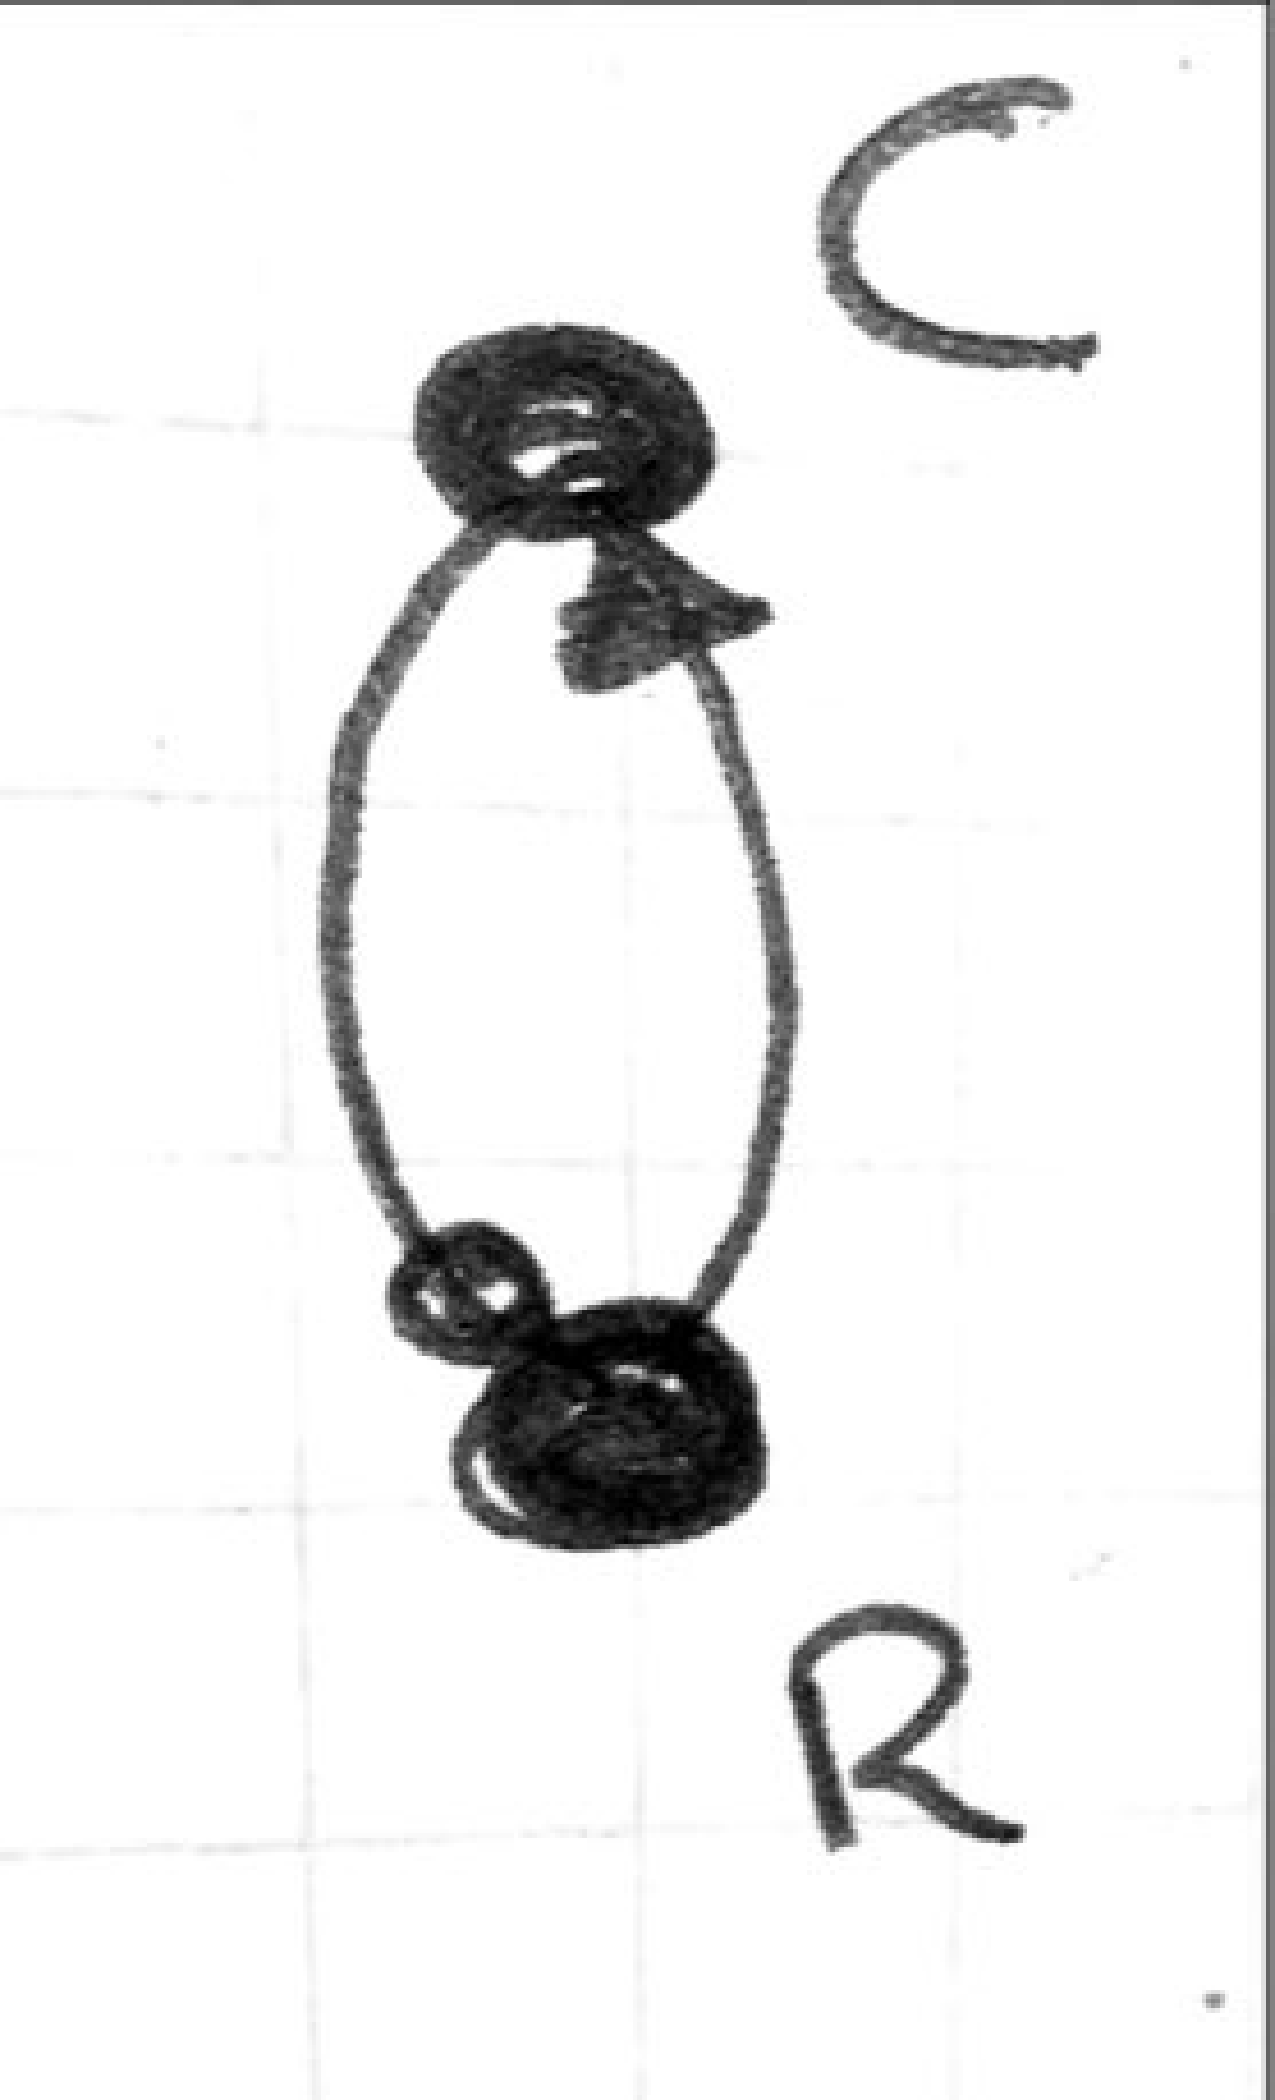
\includegraphics[width=2cm]{figs/CR_digraph.pdf}
\end{wrapfigure}
Resource is explicit:  $C$ - Consumer \& $R$ - Resource
\begin{align*}
	f_R(R,C)=\frac{dR}{dt} &= \underbrace{b \cdot R}_{\text{growth}} - \underbrace{a \cdot R \cdot C}_{\text{feeding rate}}\\
	f_C(R,C)=\frac{dC}{dt} &= \underbrace{e \cdot a \cdot R \cdot C}_{\text{conversion of prey to preds}} - \underbrace{d \cdot C}_{\text{death rate}}
\end{align*}

\textbf{What are the equilibria?}\\
\ind Prey exhibits exponential growth in absence of predators\\
\ind Predator exhibits exponential decay in absence of prey\\
\ind \ind Thus only 2:  Trivial and non-trivial (coexistence) steady state.

\textbf{Isoclines}\\
Set $f_i=0$.  Solve for $j$...
\begin{align*}
	\frac{dR}{dt} & =bR-aRC=0 \quad \Rightarrow \quad bR=aRC \quad \Rightarrow \quad C^*=\frac{b}{a}\\
	\frac{dC}{dt} & = eaRC-dC=0 \quad \Rightarrow \quad eaRC=dC \quad \Rightarrow \quad R^*=\frac{d}{ea}
\end{align*}

{
\begin{wrapfigure}{l}{0.3\textwidth}
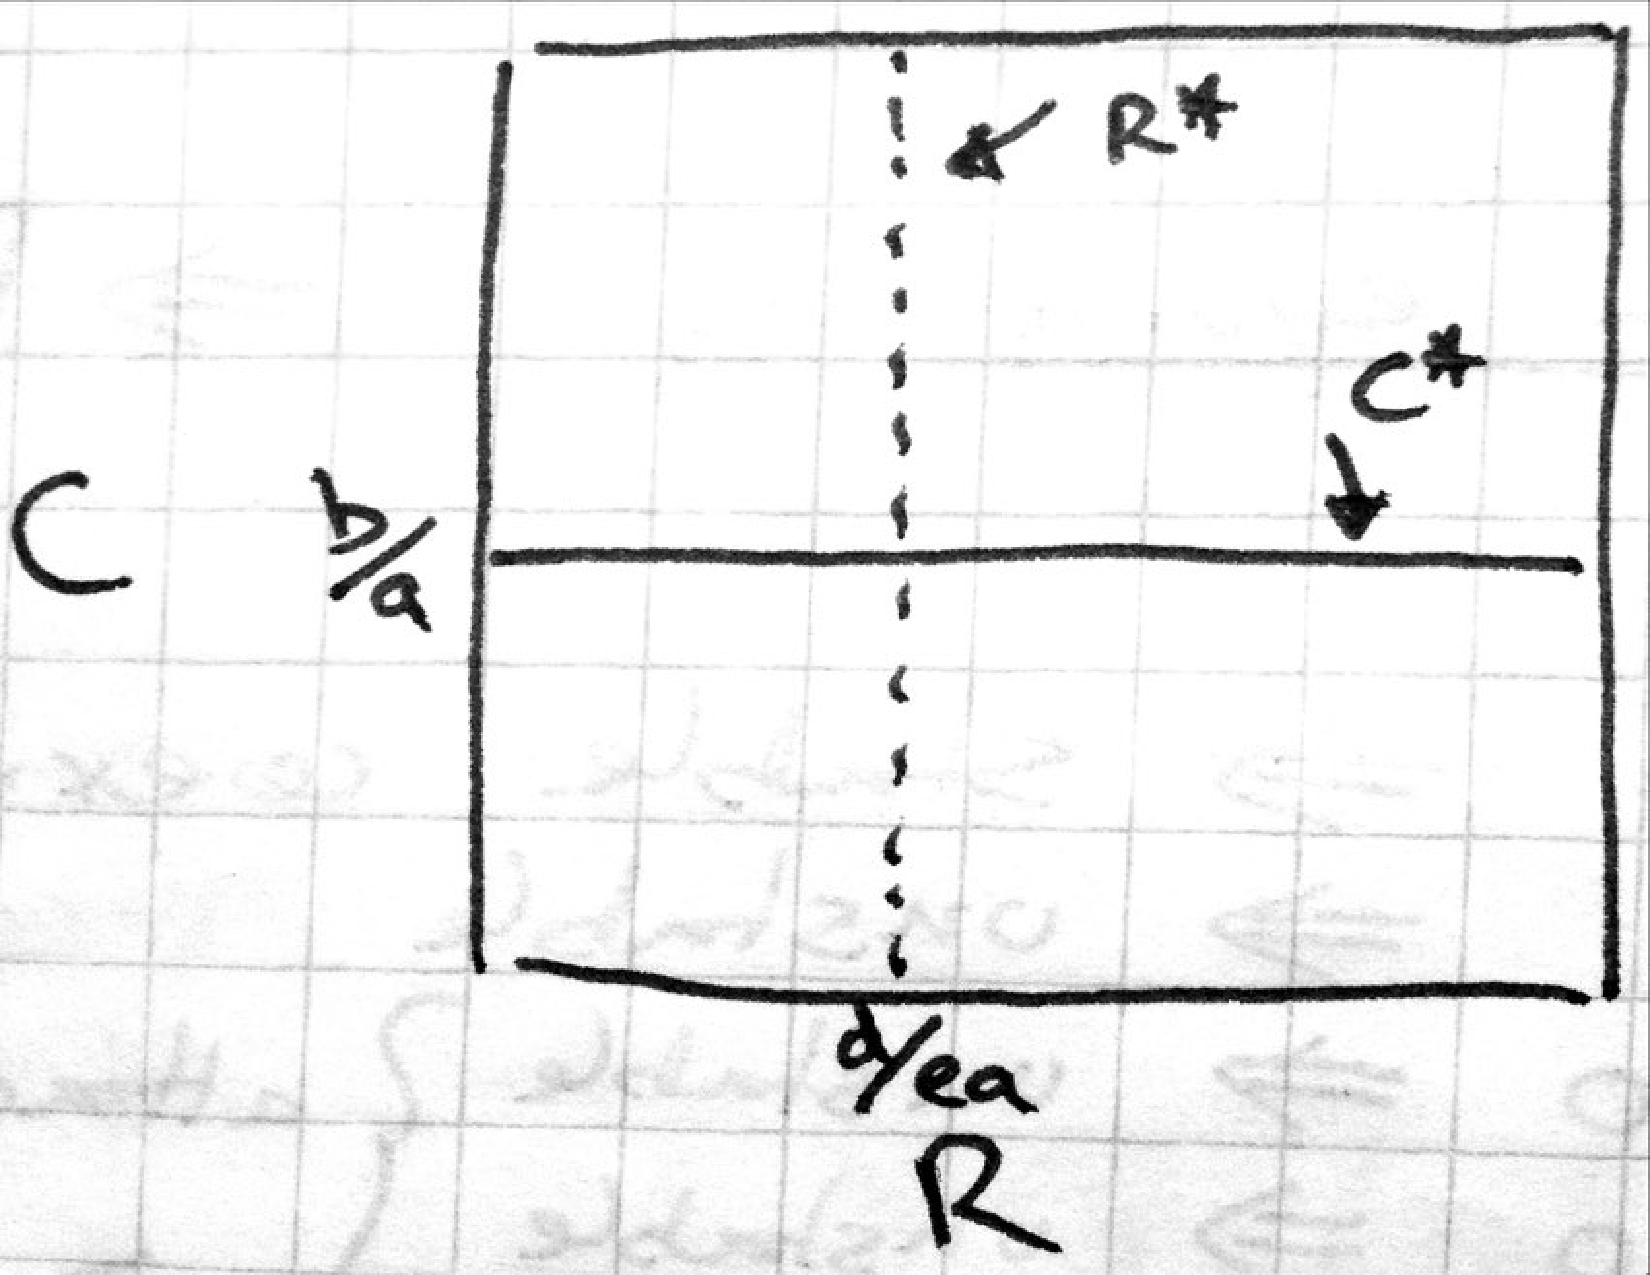
\includegraphics[width=4.5cm]{figs/LViso.pdf}
\end{wrapfigure}

Notice that both isoclines are independent of density $\Rightarrow$ straight lines!
\begin{equation*}
\begin{rcases}
  \text{If birth rate increases} & \\
  \text{or attack rate decreases} & \\
\end{rcases}
C^* \text{ increases}
\end{equation*}
\begin{equation*}
\begin{rcases}
  \text{If death rate increases} & \\
  \text{or attack rate decreases} & \\
    \text{or conversion efficiency decreases} & \\
\end{rcases}
R^* \text{ increases}
\end{equation*}

}
\ind \note{R-demonstration varying $R(0)$ and $C(0)$} \\
\ind \ind $\Rightarrow$ dependence on initial conditions. Locked phase cycle. \note{SLIDE}


\rule[0.5ex]{\linewidth}{1pt}

\pagebreak
\textbf{Stability of LV-Pred-Prey model}\\
Q: Are cycles stable or unstable?\\
\textbf{Step 1:} Construct Jacobian and evaluate at $(R^*,C^*)$.\\
\begin{equation*}
	\mathbf{A}=
	\begin{bmatrix}
		\dfrac{\partial f_R}{\partial R} & \dfrac{\partial f_R}{\partial C}\\[1em]
		\dfrac{\partial f_C}{\partial R} & \dfrac{\partial f_C}{\partial C}\\
	\end{bmatrix}
\end{equation*}

\begin{align*}
	A_{11} &= \frac{ \partial (bR-aRC)}{\partial R} = b-aC\\
		A_{12} &= \frac{ \partial (bR-aRC)}{\partial C} = -aR\\
			A_{12} &= \frac{ \partial (eaRC-dC)}{\partial R} = eaC\\
				A_{22} &= \frac{ \partial (eaRC-dC)}{\partial C} = eaR-d\\
\end{align*}
Thus
\begin{equation*}
	\mathbf{A}=
\left.	\begin{bmatrix}
		b-a C^* & -aR^*\\[1em]
		eaC^* & eaR^*-d\\
	\end{bmatrix}
	\right |_{R^*,C^*}
\end{equation*}
Then, since $C^*=\frac{b}{a}$ and $R^*=\frac{d}{ae}$...
\begin{equation*}
	\mathbf{A}=
	\begin{bmatrix}
		b-a \frac{b}{a} & -a \frac{d}{ae}\\[1em]
		ea\frac{b}{a} & ea\frac{d}{ae}-d\\
	\end{bmatrix}
	=\begin{bmatrix}
			0 & -\frac{d}{e}\\[1em]
			eb & 0\\
	\end{bmatrix}
\end{equation*}

\textbf{Step 2:} Determine eigenvalues of $\mathbf{A}$\\
\ind \note{$\Rightarrow $ R-demonstration}

\ind R-output: In this case $\quad \lambda_i = \underbrace{\text{Real part }= 0}_{\text{neutral stability}} \quad + \quad \underbrace{\text{complex part }\neq 0}_{\text{oscillations}} \quad \quad $ for both $i=1 \text{ and } 2$

\vspace{0.3cm}
\begin{center}
	$\Rightarrow$ \emph{The LV pred-prey model is `pathalogical'} $\Leftarrow$\\
	Like a pendulum swinging with no air or joint resistance.\\
	\note{SLIDE}Applicability to Lynx-Hare dynamics extremely questionable.\\
	Some Lynx-Hare cycles are clockwise!
\end{center}
\rule[0.5ex]{\linewidth}{1pt}
\textbf{Assumptions so far include:}
\begin{itemize}
\setlength\itemsep{0em}
	\item Exponential prey growth $\rightarrow$ \emph{use logistic instead}
	\item Exponential predator decays $\rightarrow$ \emph{okay}
	\item Linear functional response
	\item Linear numerical response
\end{itemize}

\textbf{Functional vs. Numerical Response}\\
In Lotka-Volterra model: \ind $e \cdot a \cdot R \cdot C$\\
\ind $a$ - `\emph{attack rate}' - per capita rate at which prey are encountered\\ 
\ind $e$ - rate at which consumed prey are converted to new predator numbers \\
\ind \ind (`\emph{conversion rate}' reflecting assimilation and production rates)

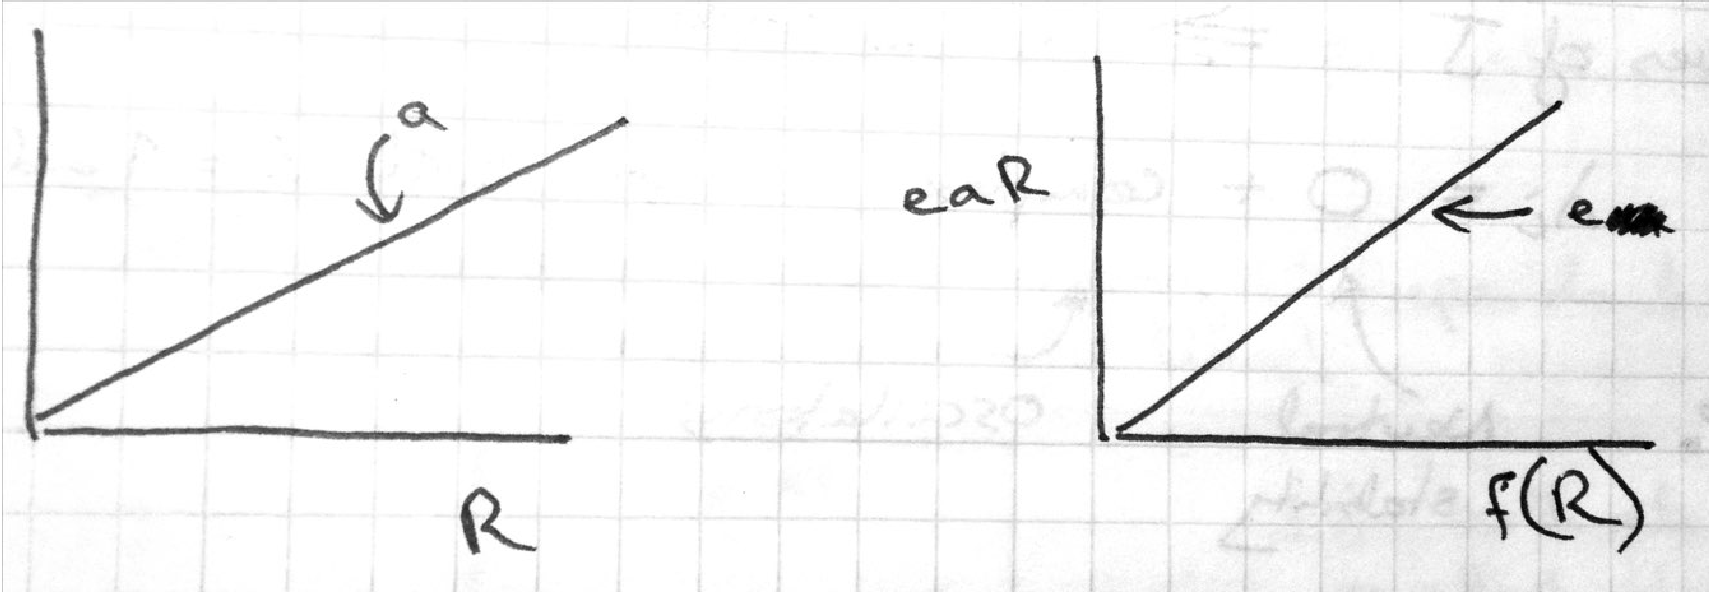
\includegraphics[width=7cm]{figs/FR_T1.pdf}
$\Rightarrow$ Feeding rate depends only on $R$ $\Rightarrow f(R)$\\

\pagebreak
Lawton, Hassell \& Beddington (1975) \note{SLIDE}
\begin{center}
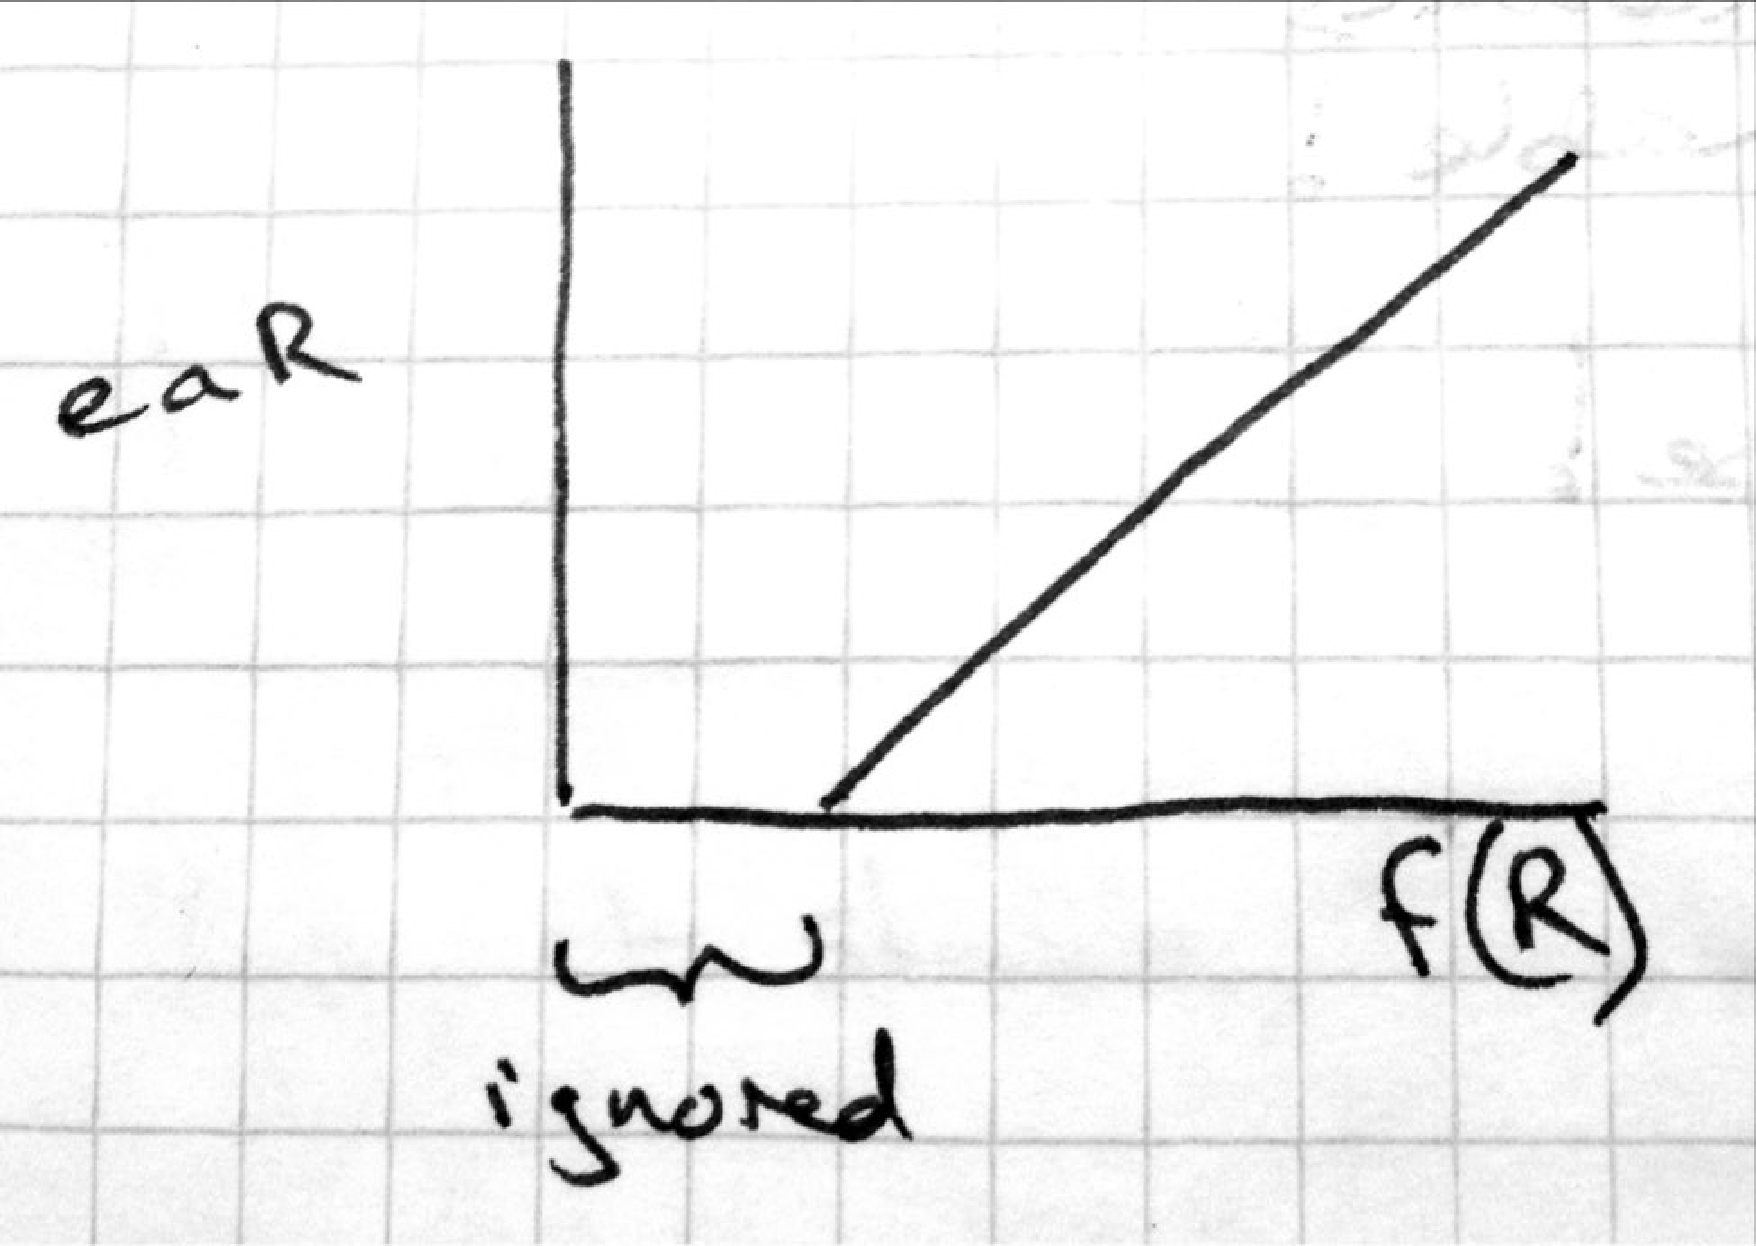
\includegraphics[width=4cm]{figs/FR_conv.pdf}
\end{center}
Linearity assumption of $e$ probably okay (but rarely tested!)

\begin{equation*}
	f(R) = a R   \quad \Rightarrow \text{ Type I functional response}. 
\end{equation*}

\textbf{Type II}\\
Is unlimited feeding rate defensible?  What limits feeding rate?

\ind Capture rate subsumed into attack rate ($a$)\\
\ind \ind - ability to search and find prey item (includes failed capture attempts)\\
\ind \emph{Handling time} ($h$) - time required to consume a successfully captured prey individual

\begin{equation*}
	f(R)=\frac{aR}{1+ahR} \quad  \Rightarrow \text{ Type II functional response}
\end{equation*}


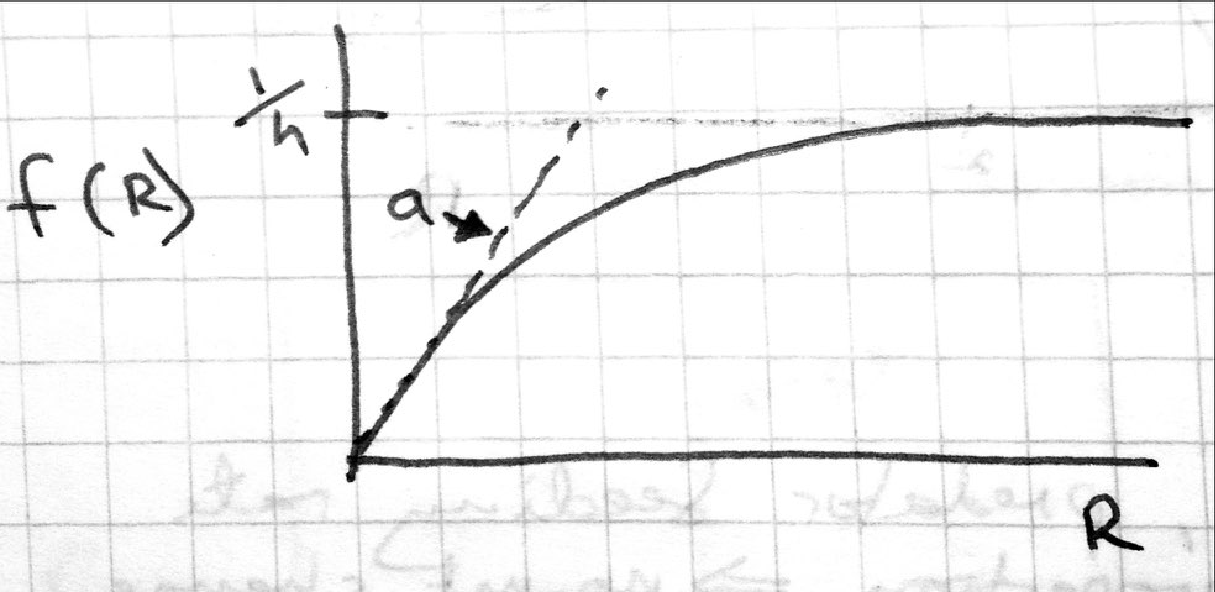
\includegraphics[width=5cm]{figs/FR_T2.pdf} \note{SLIDE}

\ind $\Rightarrow$ Saturation at high prey densities\\
\ind $\Rightarrow$ Reduces to Type I if $h=0$\\

Multi-species extension:\\
\begin{equation*}
	f(R_1,R_2)=\frac{a_1 R_1 + a_2 R_2}{1+\sum_{i=1}^2 a_i h_i R_i}
\end{equation*}

\textbf{Extension to Type III}
\begin{equation*}
	f(R)=\frac{aR^m}{1+ahR^m}
\end{equation*}
\ind If $m>1\; \Rightarrow $Type II functional response.\\
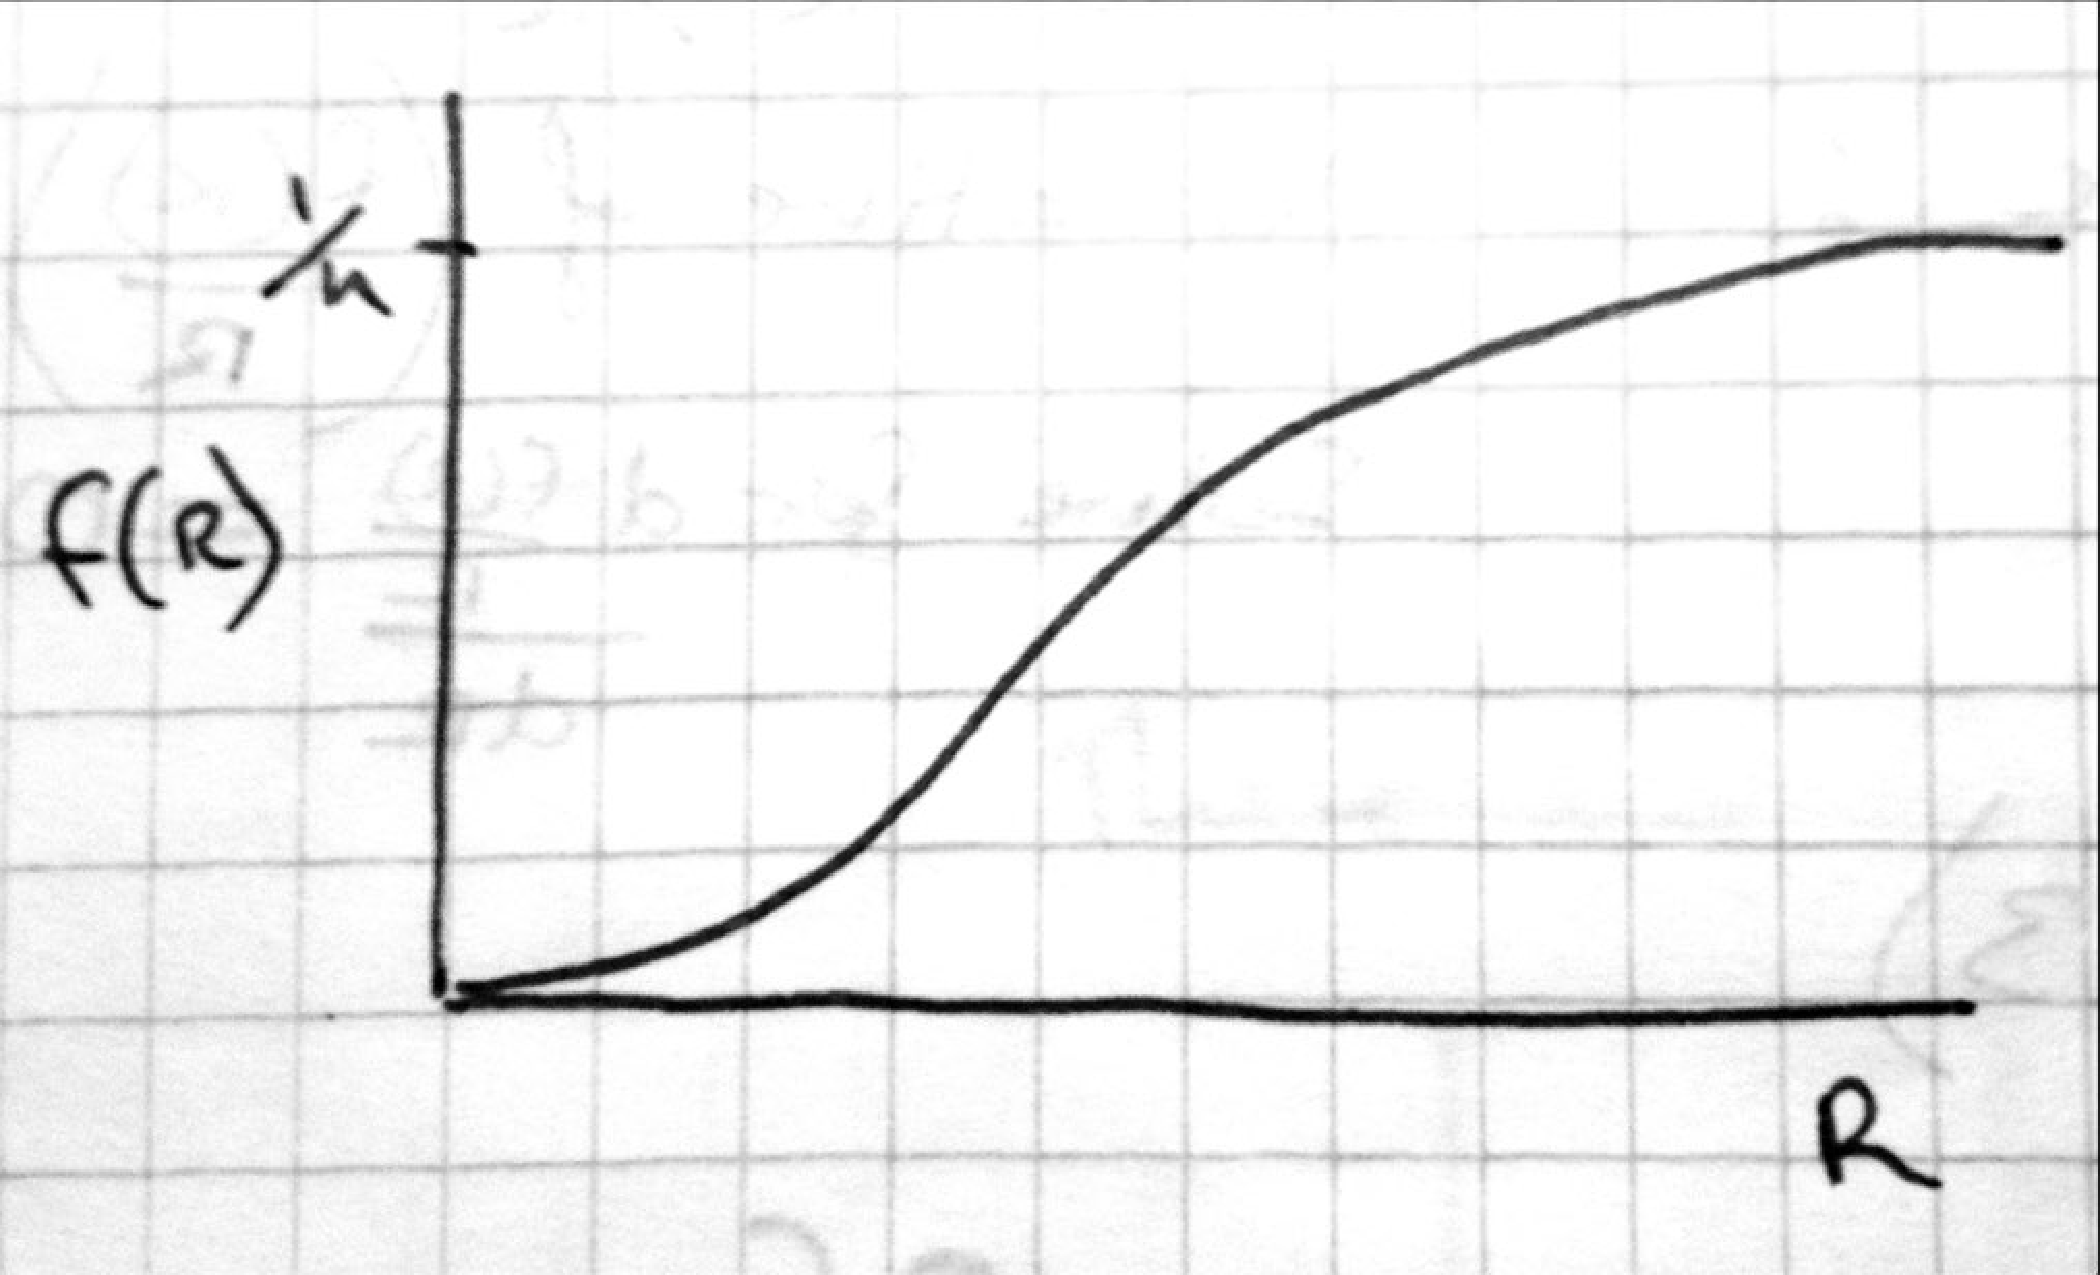
\includegraphics[width=4cm]{figs/FR_T3.pdf}

\ind $\Rightarrow$ Saturation at high prey densities\\
\ind $\Rightarrow$ Accelerating feeding rate at low prey densities\\
\ind $\Rightarrow$ Reduces to Type II if $m=1$\\
\ind $\Rightarrow$ Reduces to Type I if $m=1$ \& $h=0$\\

`Phenomenological' model of prey switching where consumer ignores focal prey at low prey densities.\\
e.g., Let $\hat{a} = aR$ (preference increases with density), then get $f(R)=\frac{aR^2}{1+ahR^2}$.\\

\note{NOTE:}  Many more functional response models exist!

\rule[0.5ex]{\linewidth}{1pt}
\pagebreak

\textbf{Effects of alternative functional responses on prey's \emph{per capita} mortality rate (i.e. $\frac{f(R)}{R}$)}
\begin{align*}
	\text{Type I: } &\frac{f(R)}{R}=\frac{aR}{R}=a \\
	\text{Type II: } & \quad \qquad \frac{a}{1+ahR} \quad \quad \text{Note: }\lim_{R \to \infty}\frac{a}{1+ahR}=0\\
	\text{Type III: } &  \qquad \quad \frac{aR^{m-1}}{1+ahR^m} \quad \quad \text{For }m=2: \quad \frac{aR}{1+ahR^2}
\end{align*}
\begin{center}
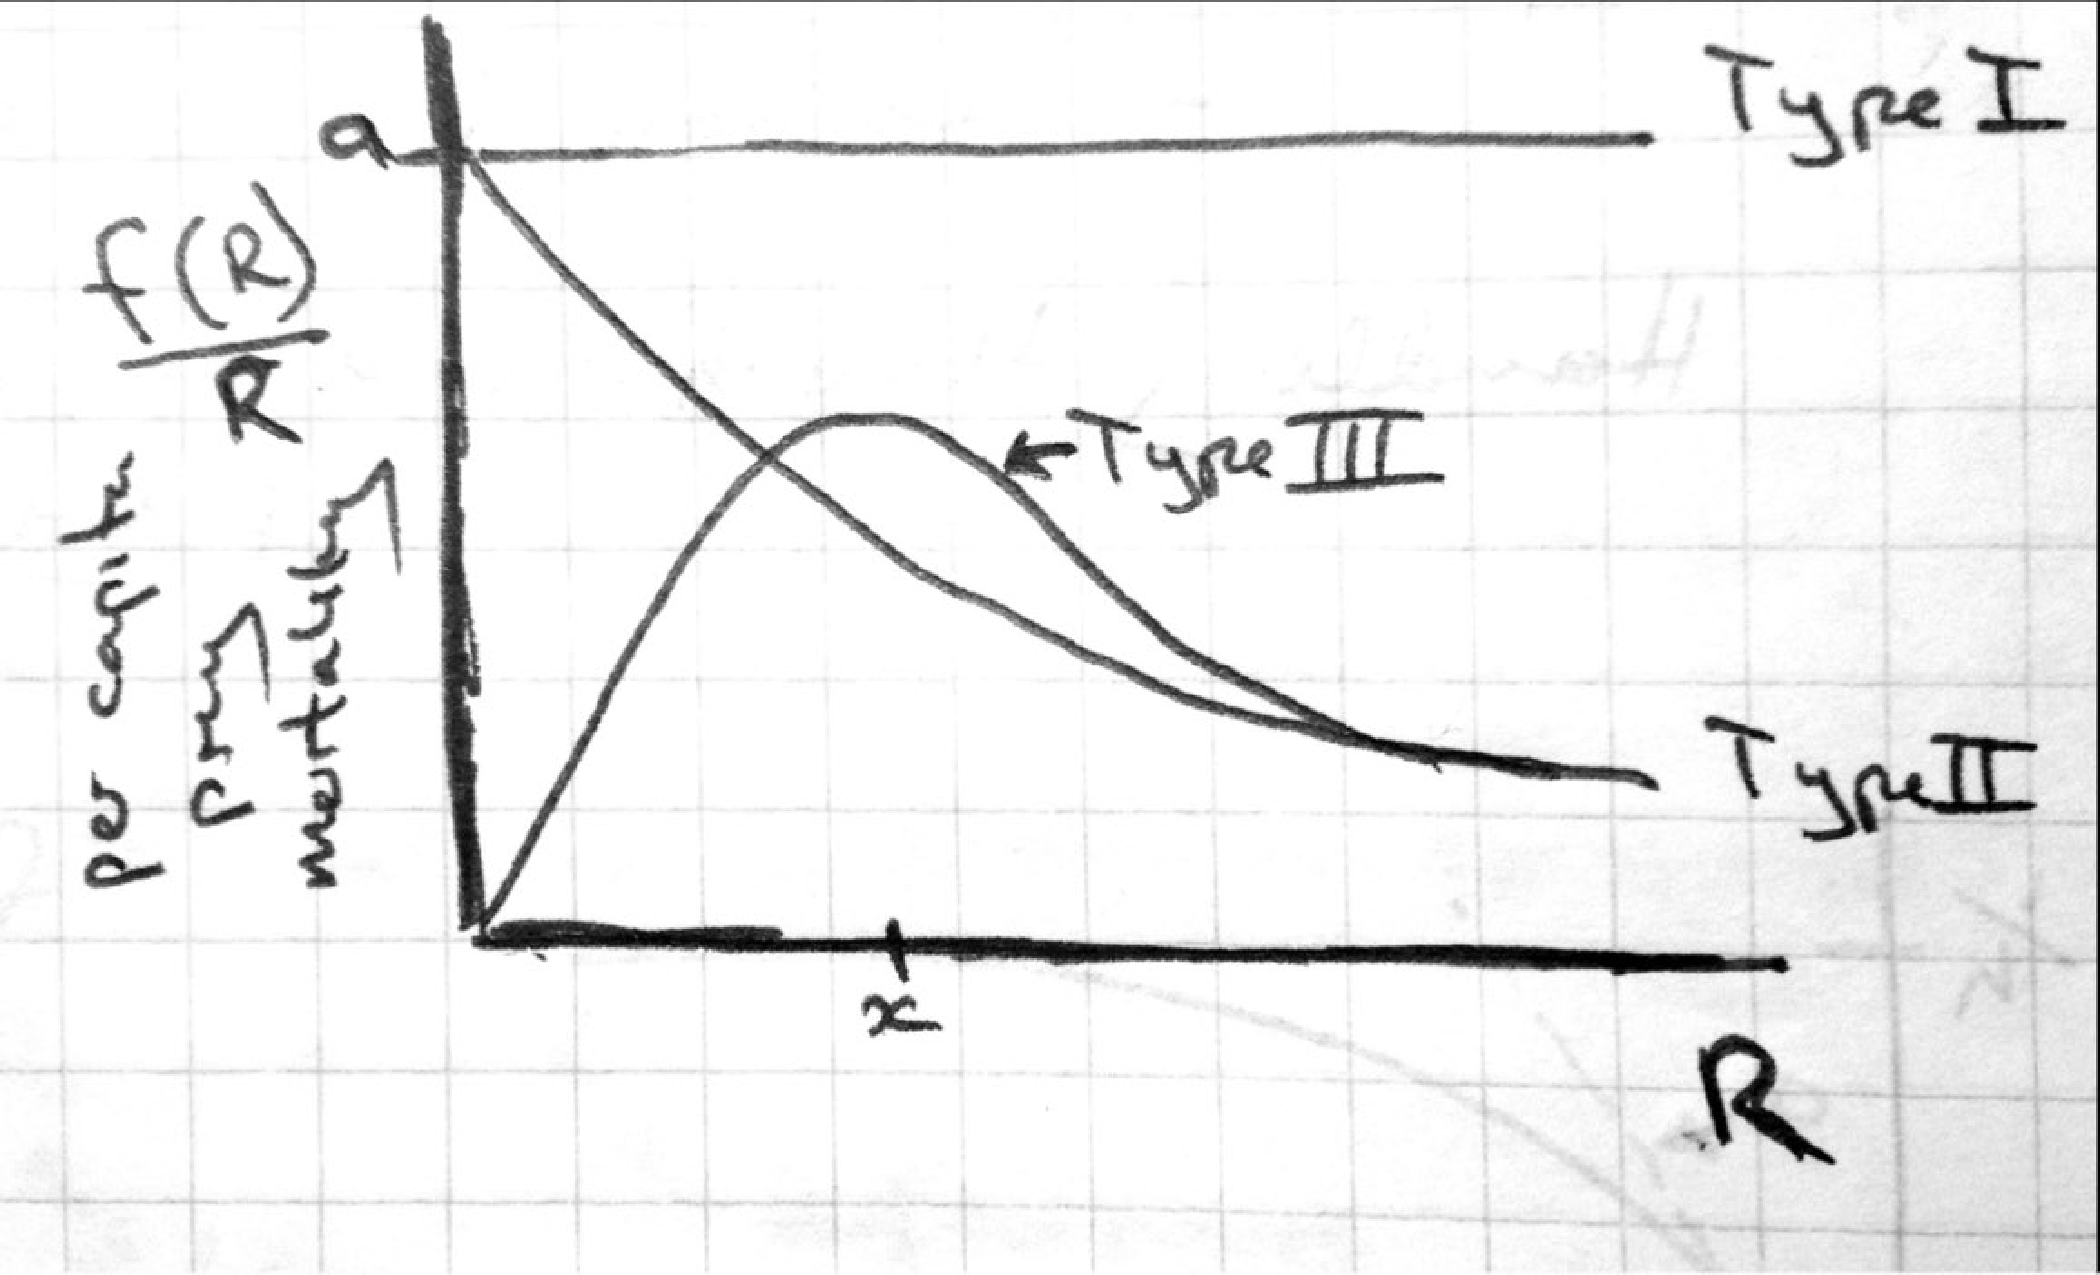
\includegraphics[width=6cm]{figs/PreyMort.pdf}
\end{center}

\textbf{Type I}: Neutral response\\
\ind \ind As prey increases, predator feeding rate increases in constant proportion $\Rightarrow$ no net change.\\
\textbf{Type II}: Prey per capita mortality rate increases as $R$ increases/ decreases as $R$ increases.\\
\textbf{Type III}: Prey experiences refuge at low $R < x$
\begin{equation*}
\frac{a  R}{1+ahR^m}
\end{equation*}
\ind \ind \ind Numerator dominates for $R<x$\\
\ind \ind \ind Denominator dominates for $R>x$\\

\note{Q:} How would you find value of $x$?
\note{A:} Solve for $x$ in derivative: $\dfrac{d \frac{f(R)}{R}}{dR}$!

\rule[0.5ex]{\linewidth}{1pt}

\begin{wrapfigure}{r}{0.2\textwidth}
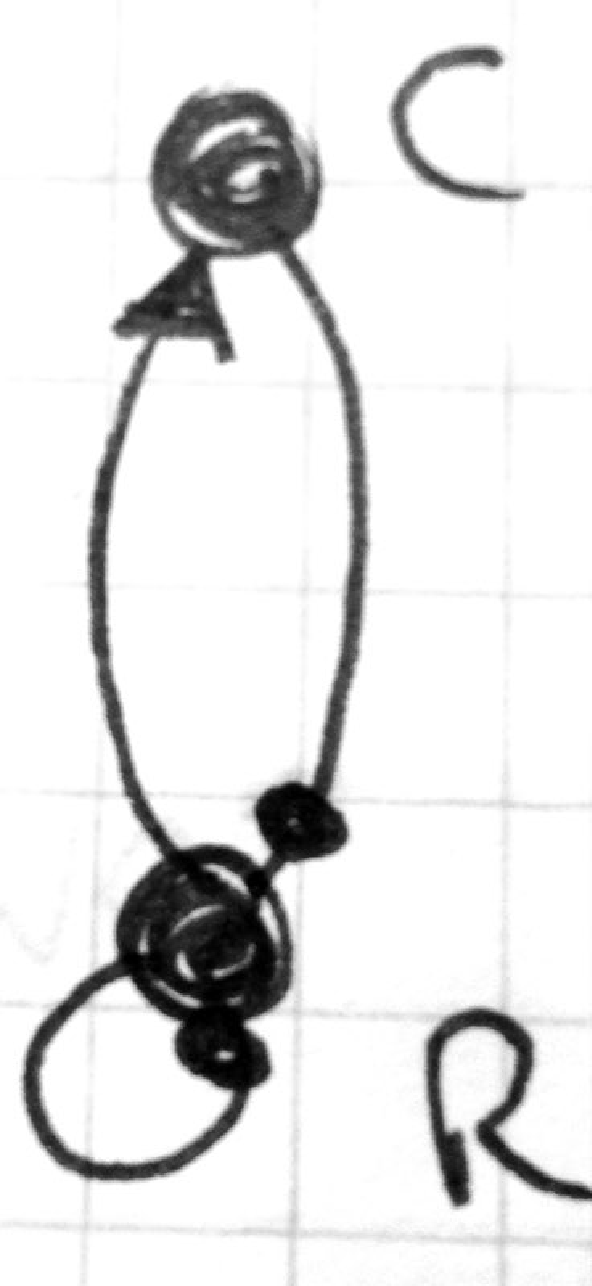
\includegraphics[width=1cm]{figs/CR_digraph2.pdf}
\end{wrapfigure}

\textbf{MacArthur-Rosenzweig Model (1963)}(a.k.a. Paradox of enrichment model)

\begin{equation*}
	\frac{dR}{dt}=bR(1-\alpha R) - \frac{aRC}{1+ahR} \qquad \qquad  \frac{dC}{dt}=\frac{eaRC}{1+ahR}-dC 
\end{equation*}

\textbf{Isoclines}\\
\ind \note{$\Rightarrow$ Mathematica}\\

Remember from LV-model:
\begin{equation*}
	R^*=\frac{d}{ae} \qquad \qquad C^* = \frac{b}{a}
\end{equation*}

For MacArthur-Rosenzweig model:
\begin{equation*}
	R^*=\frac{d}{ae-adh} \qquad \qquad C^* = \frac{b}{a} + \frac{bR(ah-\alpha-a \alpha h R)}{a}
\end{equation*}
\begin{center} $\Rightarrow$ $C^*$ depends on $R$.\end{center}

\begin{center}
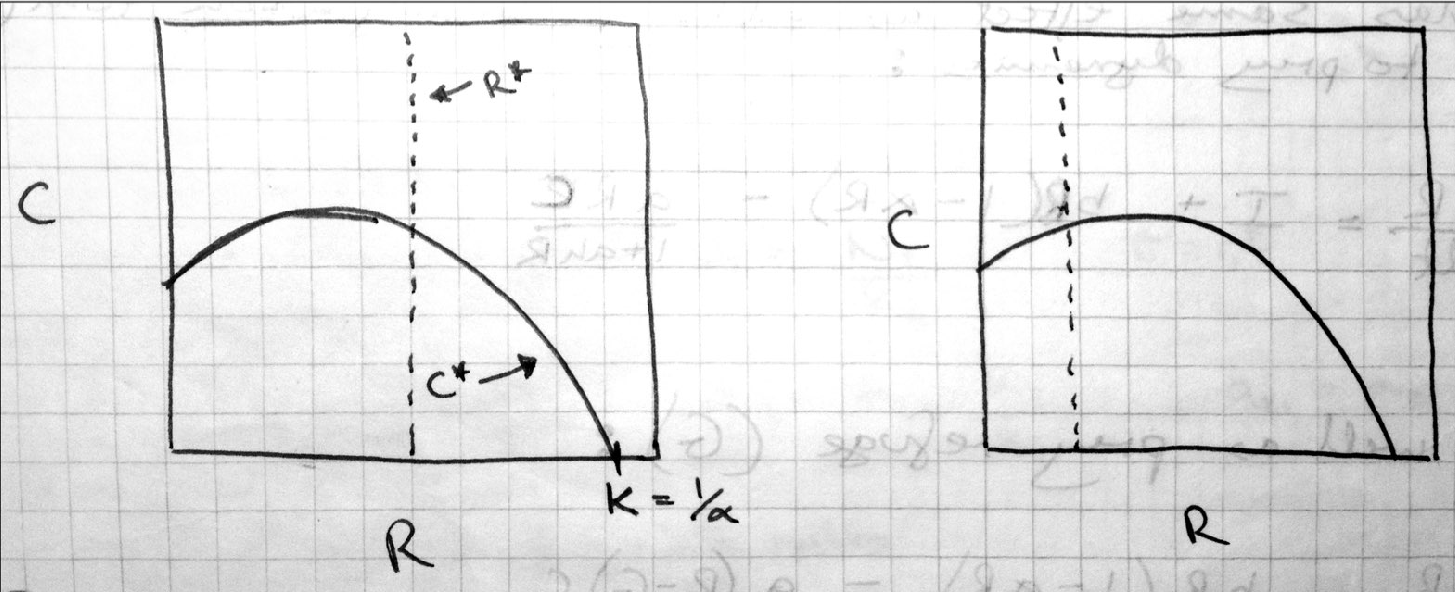
\includegraphics[width=9cm]{figs/MRiso.pdf}
\end{center}

When isoclines intersect to the \emph{right} of hump $\Rightarrow$ fixed point equilibrium\\
When isoclines intersect to the \emph{left} of hump $\Rightarrow$ limit cycles\\

\textbf{Find equilibria}\\
\ind \note{$\Rightarrow$ Mathematica}\\
Sometimes may be given \emph{four} equilibria !?!?!
\begin{center}
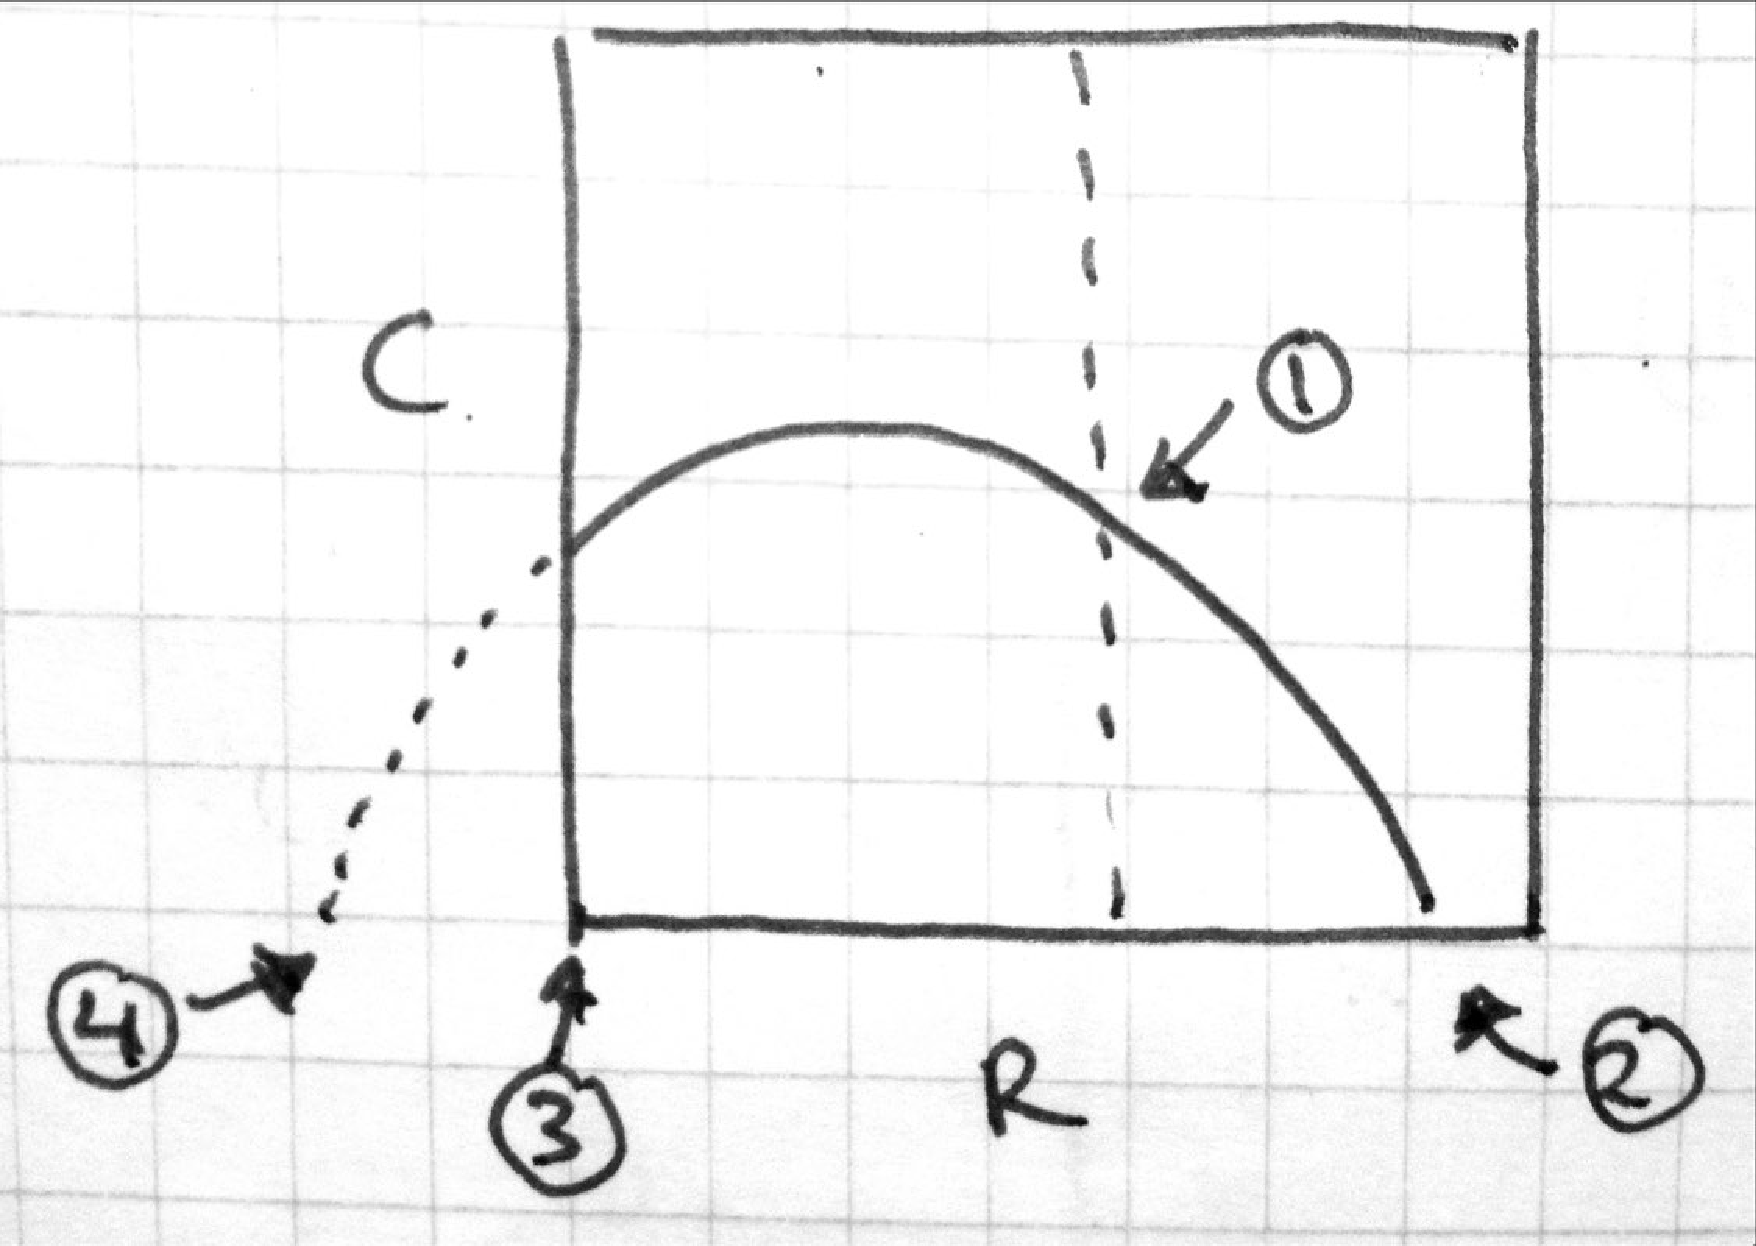
\includegraphics[width=5cm]{figs/MRiso2.pdf}
\end{center}

\ind \circled{1} $R^*>0, C^*>0$ coexistence\\
\ind \circled{2} $R^*=K, C^*=0$ boundary (invasible)\\
\ind \circled{3} $R^*=0, C^*=0$ trivial \\
\ind \circled{4} $R^*<0, C^*=0$ unfeasible\\

\textbf{Study isoclines}\\
\begin{equation*}
\begin{rcases}
  \text{decreasing }d & \\
  \text{increasing }e & \\
  \text{increasing }a & \\
\end{rcases}
	\text{ moves } R^* \text{ to left }\Rightarrow \text{ limit cycles}
\end{equation*}
\begin{equation*}
\begin{rcases}
  \text{increasing }a & \\
  \text{increasing }h & \\
  \text{increasing }b & \\
  \text{decreasing } \alpha & \\
\end{rcases}
\uparrow
\text{ steepness and moves hump to right }\Rightarrow \text{ limit cycles} 
\end{equation*}

\note{SLIDE:}\\
\ind Luckinbill (1973) experiment manipulated $a$ $\Rightarrow$ cycles or extinction\\
\ind Decreasing $\alpha$ (i.e. increasing $K$) $\Rightarrow$ `Paradox of enrichment'

\rule[0.5ex]{\linewidth}{1pt}

\textbf{Isoclines of Type III (Problem set \#6)}\\
\begin{center}
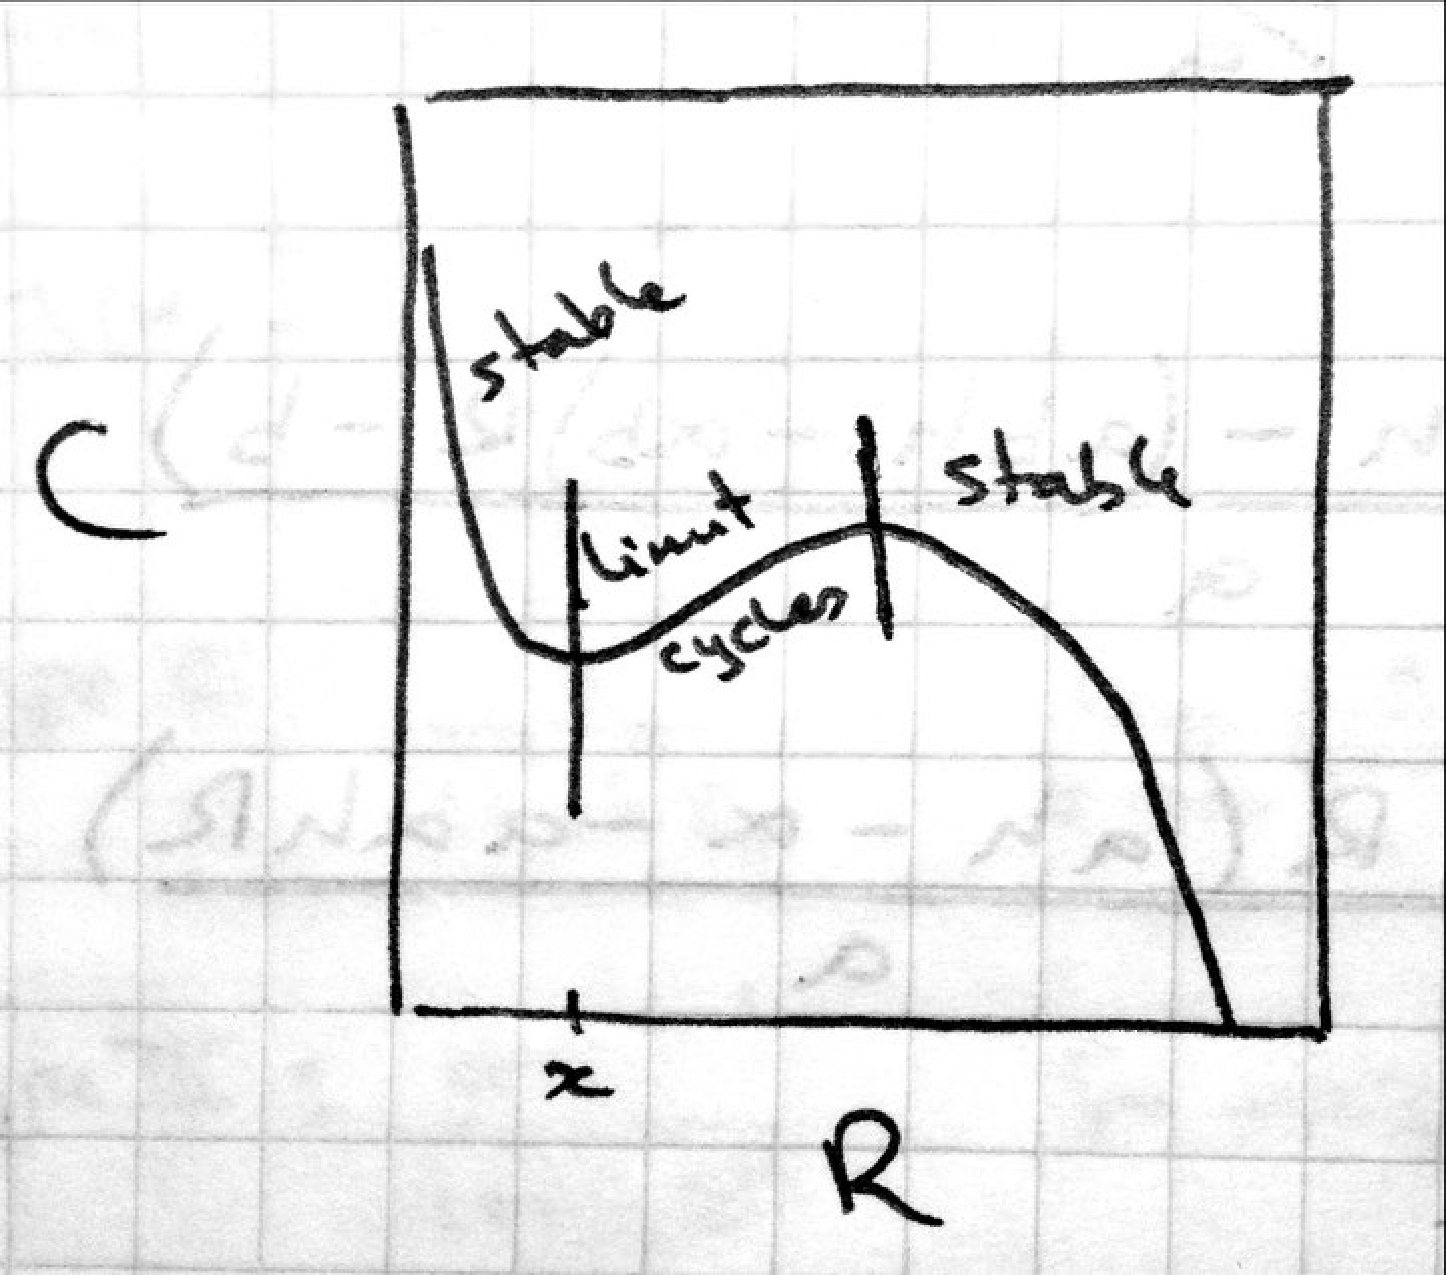
\includegraphics[width=5cm]{figs/MRiso3.pdf}
\end{center}

Type III has same effect as adding Immigration term ($I$) to prey growth...
\begin{equation*}
	\frac{dR}{dt}=I+bR(1-\alpha R) - \frac{aRC}{1+ahR}
\end{equation*}
...as well as the effect of adding a prey refuge ($R'$)...
\begin{equation*}
	\frac{dR}{dt}=bR(1-\alpha R) - \frac{a(R-R')C}{1+ah(R-R')} \qquad \qquad \frac{dC}{dt}=\frac{ea(R-R')C}{1+ah(R-R')} - dC
\end{equation*}


\rule[0.5ex]{\linewidth}{1pt}


\end{document}